\section{Priority Model}

For a given problem, we assume that the input items belong to some set $\mathcal{J}$. For any execution of the algorithm, the input is a finite subset $\mathcal{I} \subset \mathcal{J}$.

Let $f:\,\mathcal{J} \to \R$ be a function. We do not place restriction on the complexity or computability of such function. For an input set $\mathcal{I} = \{I_1,\ldots,I_n\}$, the function induces a total ordering $\preceq$ on $\mathcal{I}$, breaking ties using certain rules (for example, by input ID).

For a fixed order priority algorithm, $f$ and $\preceq$ are set initially before the algorithm observes the input set. For adaptive order, the algorithm computes $f$ and $\preceq$ dynamically. More formally, there is a different function $f_i$ and ordering $\preceq_i$ associated with each iteration $i$ where $f_i$ and $\preceq$ depends on the items $\{I_1,\ldots,I_{j}\}$ considered in prior iterations $j < i$. 

Let us first consider fixed order algorithm under this priority model. In each iteration $k$ for $1 \leq k \leq n$, the algorithm observes input element $I_k \in \mathcal{I}$ and based on this input and all previous inputs and decisions, the algorithm makes an irrevocable decision $D_k$ about this input item (this typically involves whether to include or discard the current item).

This model gives us the following template for fixed order priority algorithms

\begin{codebox}
    \li $\mathcal{J} =$ set of all possible inputs
    \li $\preceq\,\, = $ a total ordering on $\mathcal{J}$ (typically induced by a function $f$)
    \li $\mathcal{I} \subset \mathcal{J} = $ actual input to the algorithm
    \li $S = \emptyset$ \RComment{items already examined by the algorithm}
    \li $i = 0$
    \li \While $\mathcal{I} - S \neq \emptyset$ \Do
        \li $i = i + 1$
        \li $\mathcal{I} = \mathcal{I} - S$
        \li $I_i = \min_{\preceq} \{ I \in \mathcal{I} \}$ \RComment{select min element based on the ordering $\preceq$}
        \li make an irrevocable decision $D_i$ concerning $I_i$ 
        \li $S = S \cup \{I_i\}$
    \End      
\end{codebox}

This template can be modified to allow the algorithm to determine the total ordering dynamically based on the elements it has observed so far.

\begin{codebox}
    \li $\mathcal{J} =$ set of all possible inputs
    \li $\mathcal{I} \subset \mathcal{J} = $ actual input to the algorithm
    \li $S = \emptyset$ \RComment{items already examined by the algorithm}
    \li $i = 0$
    \li \While $\mathcal{I} - S \neq \emptyset$ \Do
        \li $i = i + 1$
        \li $\preceq_i\,\, = $ a total ordering on $\mathcal{J}$ (typically induced by a function $f_i$)
        \li $\mathcal{I} = \mathcal{I} - S$
        \li $I_i = \min_{\preceq_i} \{ I \in \mathcal{I} \}$ \RComment{select min element based on the ordering $\preceq_i$}
        \li make an irrevocable decision $D_i$ concerning $I_i$ 
        \li $S = S \cup \{I_i\}$
        \li $\mathcal{J} = \mathcal{J} - \{I \in \mathcal{I} \mid I \preceq_i I_i \}$
    \End      
\end{codebox}

For greedy algorithm, the algorithm does not have knowledge of the input other than the elements it has observed so far. Sometimes, we allow the algorithm to have some easily computed global information such as the size of the input. The input is said to be chosen by an adversary.

This generalization applies to a broader category of algorithms known as priority-based algorithms. Informally, greedy algorithms always assume that the current iteration could be the last one and the current item being considered might as well be the last item. Hence, an optimal decision is immediate when the algorithm finishes. A more general priority algorithm that are not necessarily greedy does not have such restriction

This formalization was first given by Allan Borodin \textit{et al.} in \textit{(Incremental) Priority Algorithms} (Thirteen Annual ACM-SIAM Symposium on Discrete Algorithms, January 2002) \cite{borodin-priority}.

\section{Global Optimality of Greedy Algorithms}

(From Allan Borodin's notes)

Most greedy algorithms are not opitmal. The method we use to show that a greedy algorithm is optimal (when it is) known as the exchange argument often proceeds as follws. At each stage $i$, we define our partial solution to be promising if it can be extended to an optimal solution by using elements that haven't been considered yet by the algorithm; that is, a partial solution is promising after stage $i$ if there exists an optimal solution that is consistent with all the decisions made through stage $i$ by our partial solution. We prove the algorithm is optimal by fixing the input problem, and proving by induction on $i \geq 0$ that after stage $i$ is performed, the partial solution obtained is promising. The base case of $i=0$ is usually completely trivial: the partial solution after stage O is what we start with, which is usually the empty partial solution, which of course can be extended to an optimal solution. The hard part is always the induction step, which we prove as follmvs. Say that stage $i+1$ occurs, and that the partial solution after stage $i$ is $S_i$ and that the partial solution after stage $i+1$ is $S_{i+1}$, and we know that there is an optimal solution $S_{opt}$ that extends $S_i$; we want to prove that there is an optimal solution $S_{opt}'$ that extends $S_{i+1}$. $S_{i+1}$ extends $S_i$ by taking only one decision; if $S_{opt}$ makes the same decision, then it also extends $S_{i+1}$, and wve can just let $S_{opt}' = S_{op}$ and we are done. The hard part of the induction step is if $S_{opt}$ does not extend $S_{i+1}$, In this case, we have to show either that $S_{opt}$ could not have been optimal (implying that this case cannot happen), or we show how to change some parts of $S_{opt}$ to create a solution $S_{opt}'$ such that

\begin{itemize}
    \item $S_{opt}'$ extends $S_{i+1}$ and
    \item $S_{opt}'$ has value (cost, profit, etc.) at least as good as $S_{opt}$, so the fact that $S_{opt}$ is optimal implies that $S_{opt}'$ is optimal.
\end{itemize}

For most greedy algorithms, when it ends, it has constructed a solution that cannot be extended to any solution other than itself. Therefore, if we have proven the above, we know that the solution constructed by the greedy algorithm must be optimal.

\section{Greedy v.s. DP}

In the next part, we will examine dynamic programming, which is another powerful algorithm design paradigm for solving many optimization problem. In fact, greedy and dynamic programming shares a lot of similarities, especially in the sense that both approaches exploit the optimal substructure property where the globally optimal solution can be constructed from optimal solutions of its subproblems.

Unlike greedy, which makes the locally optimal choice, dynamic programming solves potentially overlapping subproblems and makes an informed choice.

The major differences can be summarized using this chart

\begin{table}[htbp]
    \centering\begin{tabular}{p{0.18\textwidth}|p{0.3\textwidth}|p{0.3\textwidth}}
        & Greedy & DP \\
        \hline
        Decision & starts from minimal subproblem, construct solution based on best option for the current step & starts from minimal subproblem, recursively construct solution based on all previously considered subproblems; use memoization for overlapping subproblems \\
        \hline
        Optimality & not necessarily & yes \\
        \hline
        Space complexity & better & requires an array to store solutions previously considered subproblems \\
        \hline
        Time complexity & usually better & usually polynomial \\
        \hline
        Examples & Kruskal and Prim; Dijkstra; interval scheduling (selection) and partition (coloring) & Bellman-Ford; 0-1 knapsack; longest common subsequence
    \end{tabular}
    \caption{Differences between greedy and dynamic programming}
    \label{tab:greedy-vs-dp}
\end{table}

Another way to view greedy and dynamic programming is to consider the problem and the possible solutions as a set and compare how the two approaches reduce the size of problem and narrow down the solution space. This is an illustration that I came up completely by myself. Although it seems to make sense, it is not presented in any research articles or texts. It should only be used as an intuition to understand the similarity and differences of the two approaches and should not in any way be considered a rigorous formulation or analysis.

\begin{figure}[htbp]
    \centering
    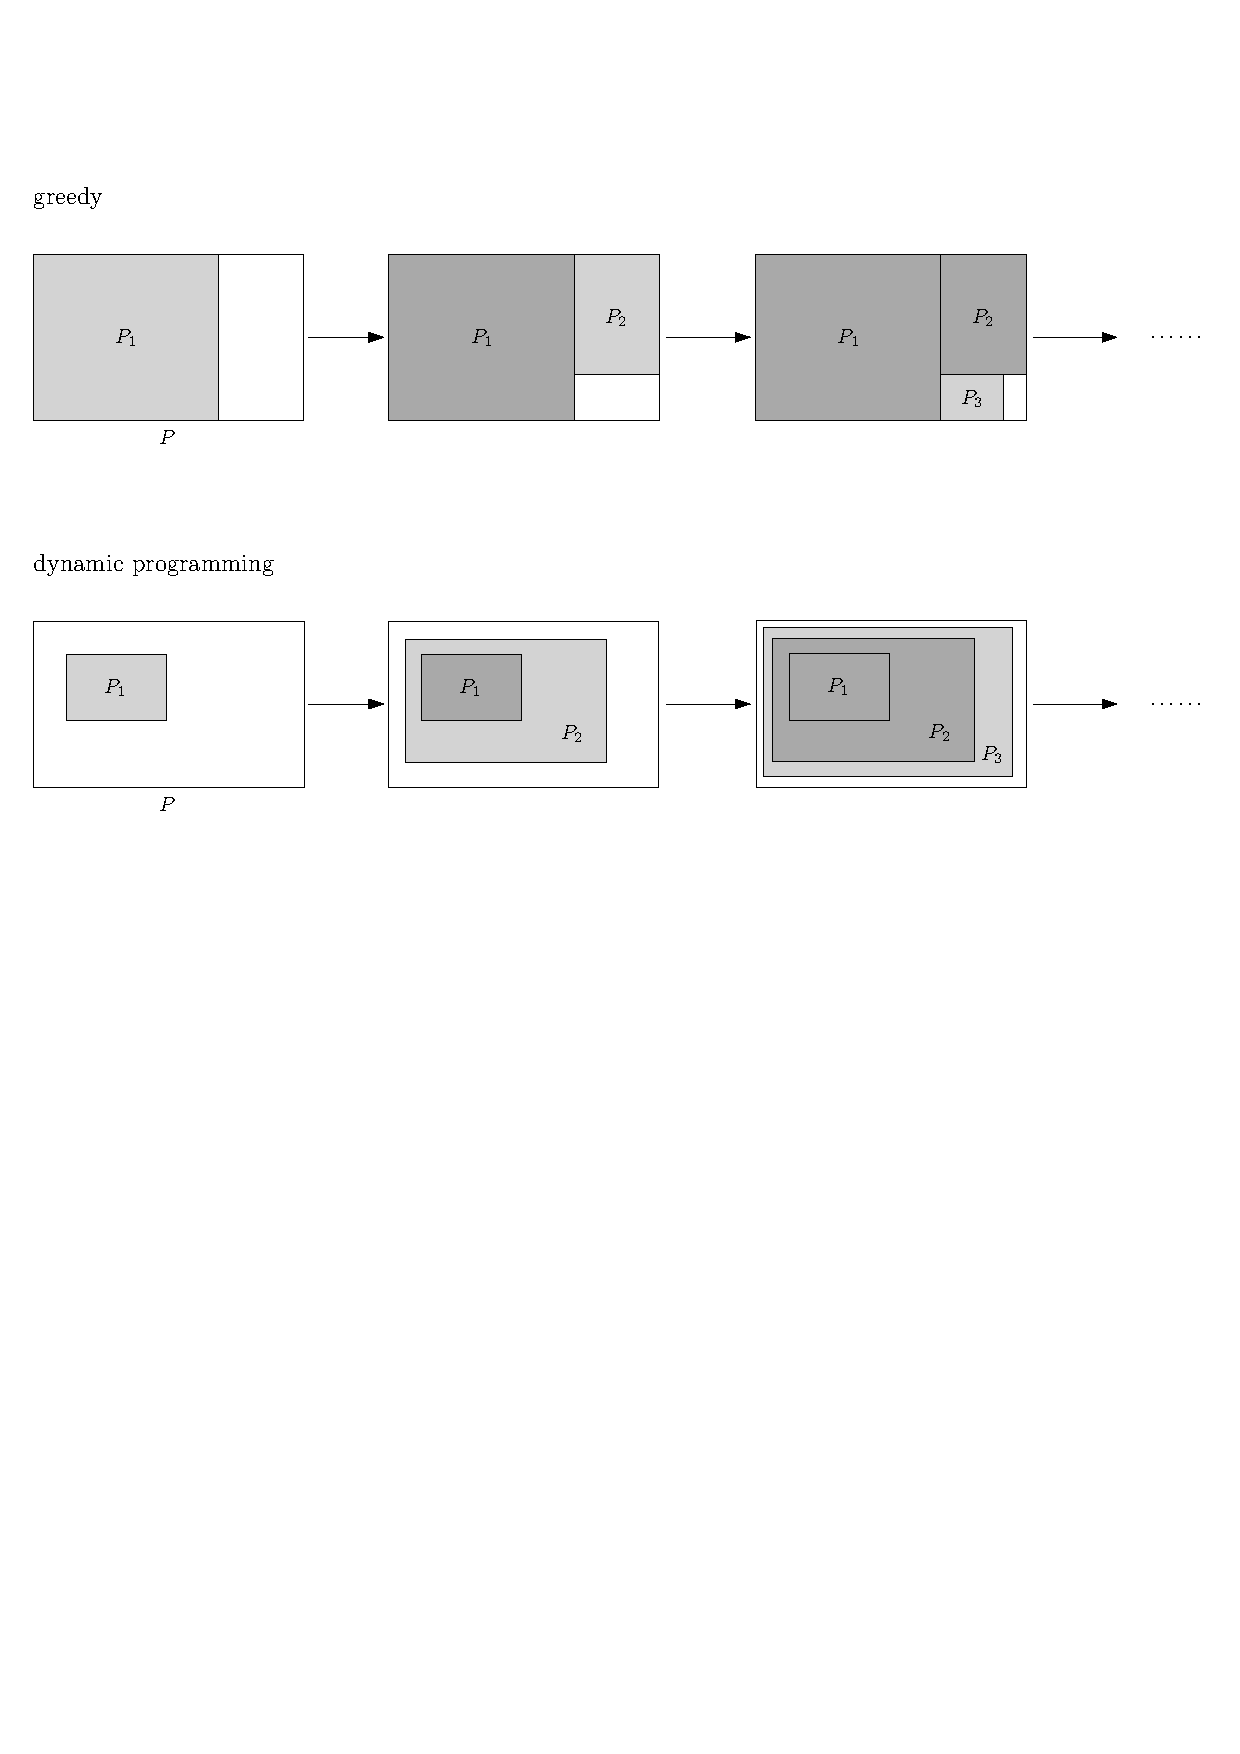
\includegraphics[width=0.9\linewidth]{dp/dp-vs-greedy.pdf}
    \caption{Another way to view the differences between greedy and DP. The rectangle represents the overall problem. Shaded region of the rectangle represents the subproblems being considered, and heavily shaded regions of the rectangle represent the subproblems that have already been solved. Note that greedy expands the solution (and reduces the size of the problem remaining) by looking at the locally optimal choice without going back; while DP often involves overlapping subproblems where a subproblem or subproblems can be contained within another subproblem (this is why memoization is important for DP).}
    \label{fig:greedy-vs-dp-set}
\end{figure}